\begin{Exercise}[title=Sismographe]
	On considère un capteur d'amplitude constitué d'un support et une masse $m$ reliés par un ressort et un amortisseur en parallèle. L'amortisseur exerce en $A$ : $\vec{F_A}=-h(\vec{v_A}-\vec{v_B})$\\
	On suppose que le support est solidaire du carter d'une machine anime d'un mouvement sinusoïdal vertical $x_1= b\sin \omega t$ par rapport au référentiel galiléen $\mathcal{R}_0 (Oxy)$
	\begin{center}
		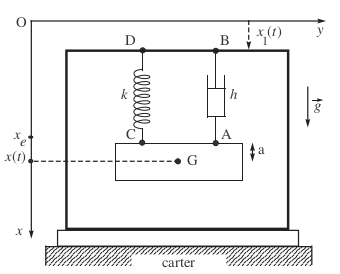
\includegraphics[scale=0.4]{../fig/sismographe.png}
	\end{center}
	\Question Déterminer l'équation que vérifie $x_e$ position de la masse à l'équilibre.
	\Question Déterminer l'équation du mouvement de $m$ dans R, mettre cette dernière sous forme canonique et la résoudre.
\end{Exercise}
\begin{Answer}
	\Question $m x'' = -k(x-x_1-l_0) - h(x'-x_1')-mg$
	\Question On a à l'équilibre: $x''=x' =0$ et $x_1 = x_1' = 0$ donc
	$x_e=l_0 -\frac{mg}{k} $
\end{Answer}
